\documentclass{standalone}
\usepackage{tikz}
\usetikzlibrary{patterns, positioning}
\usepackage[sfdefault]{ClearSans} %% option 'sfdefault' activates Clear Sans as the default text font
\usepackage[T1]{fontenc}

\begin{document}
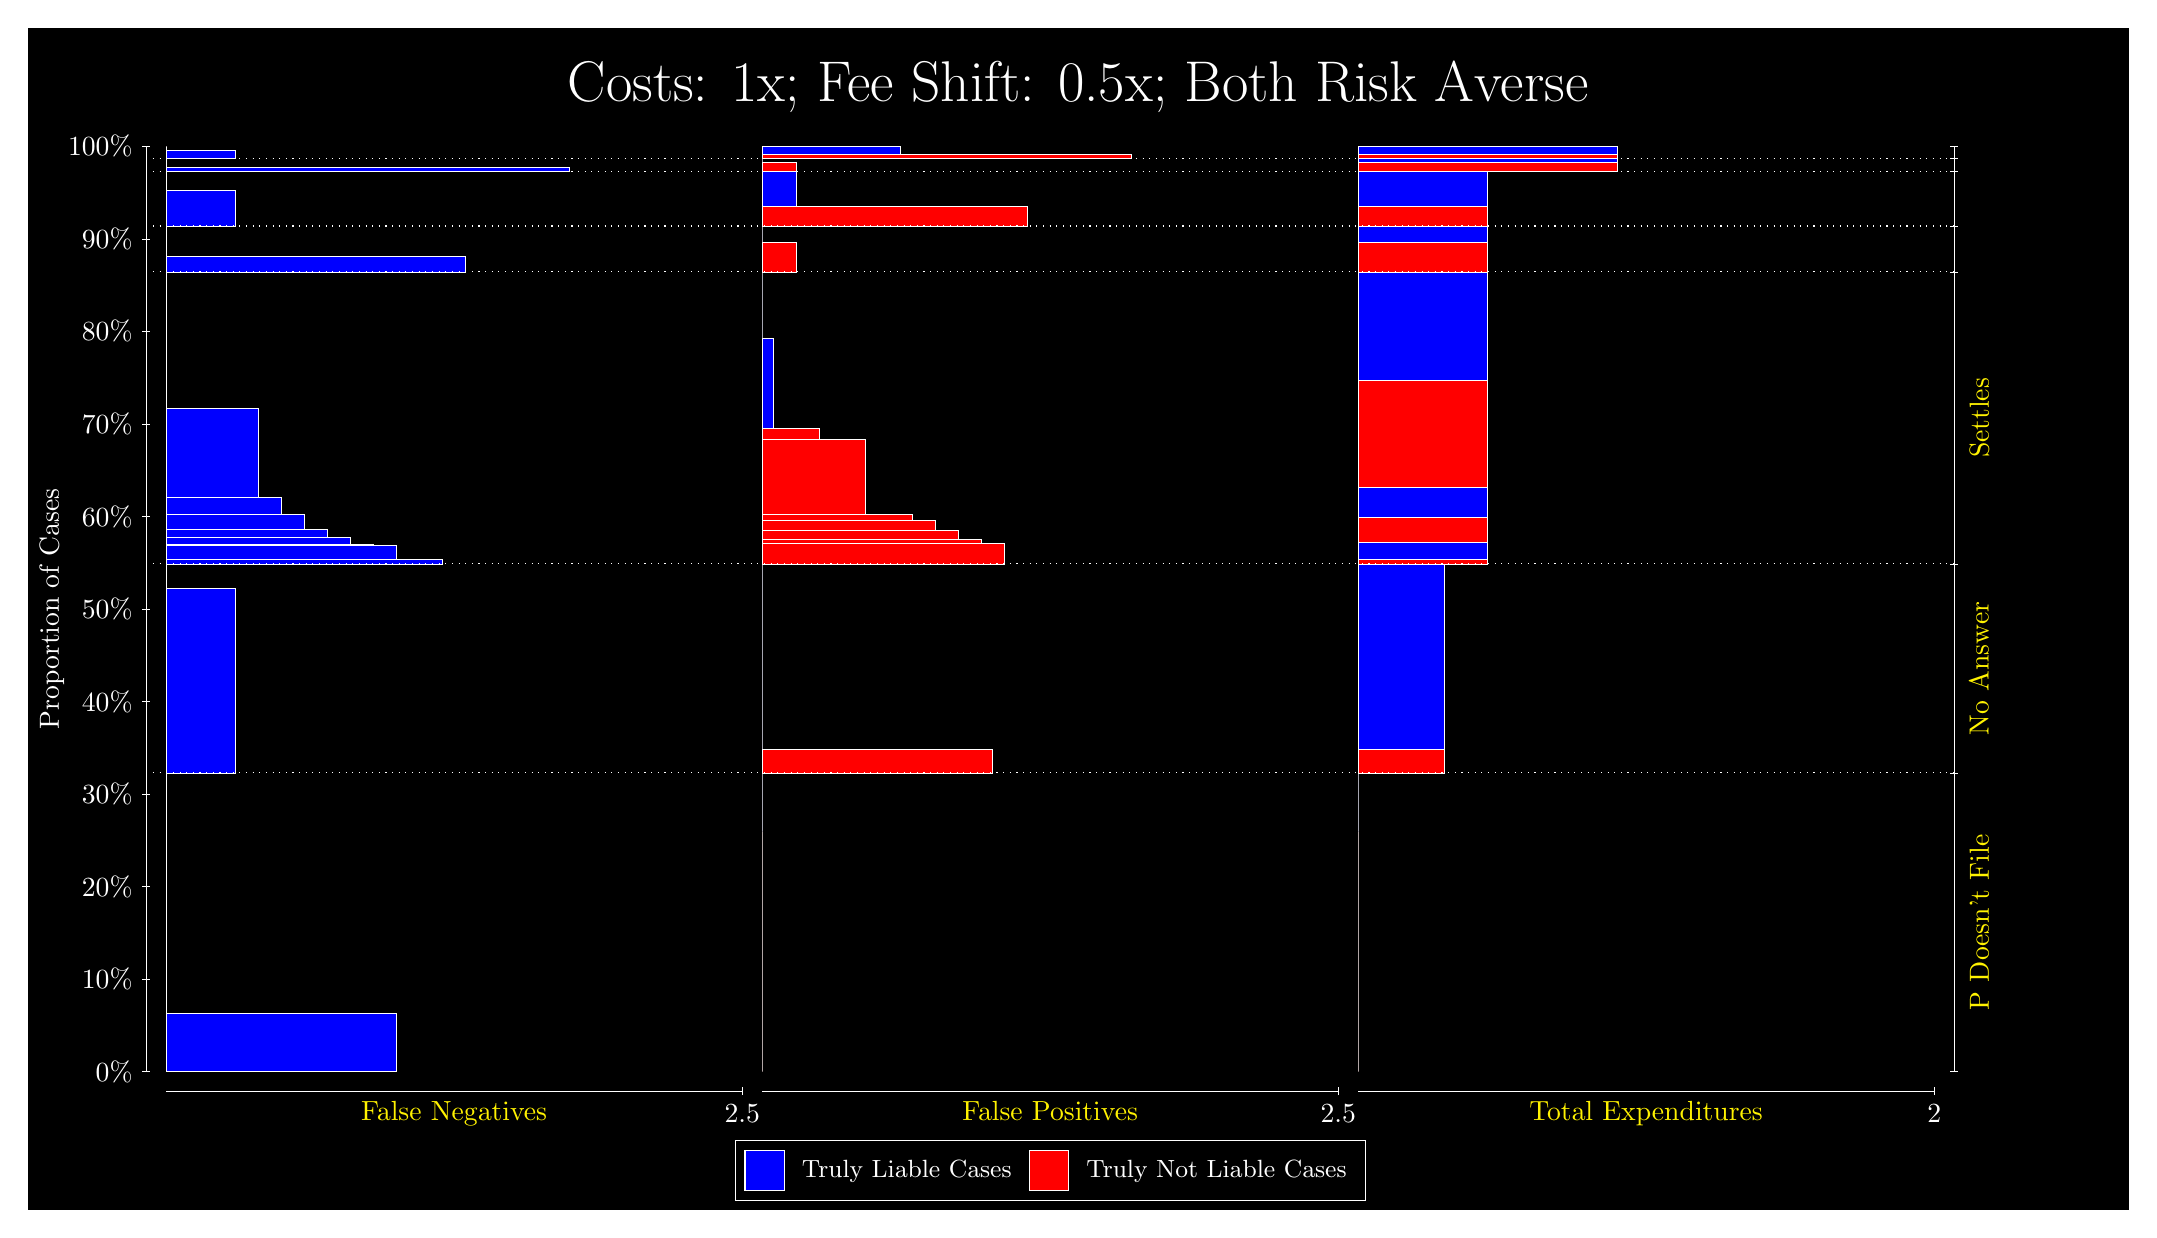
\begin{tikzpicture}
\draw[fill=black] (0,0) rectangle (26.667,15);
\draw[text=white] (0,13.5) rectangle (26.667,15) node[midway] {\huge Costs: 1x; Fee Shift: 0.5x; Both Risk Averse};
\draw[white, very thin] (1.5,1.75) -- (1.5,13.5);
\node[rotate=90, text=white, anchor=center] at (0.3, 7.625) {Proportion of Cases};
\draw[white, very thin] (1.45,1.75) -- (1.55,1.75);
\node[text=white, anchor=east] at (1.45, 1.75) {0\%};
\draw[white, very thin] (1.45,2.925) -- (1.55,2.925);
\node[text=white, anchor=east] at (1.45, 2.925) {10\%};
\draw[white, very thin] (1.45,4.1) -- (1.55,4.1);
\node[text=white, anchor=east] at (1.45, 4.1) {20\%};
\draw[white, very thin] (1.45,5.275) -- (1.55,5.275);
\node[text=white, anchor=east] at (1.45, 5.275) {30\%};
\draw[white, very thin] (1.45,6.45) -- (1.55,6.45);
\node[text=white, anchor=east] at (1.45, 6.45) {40\%};
\draw[white, very thin] (1.45,7.625) -- (1.55,7.625);
\node[text=white, anchor=east] at (1.45, 7.625) {50\%};
\draw[white, very thin] (1.45,8.8) -- (1.55,8.8);
\node[text=white, anchor=east] at (1.45, 8.8) {60\%};
\draw[white, very thin] (1.45,9.975) -- (1.55,9.975);
\node[text=white, anchor=east] at (1.45, 9.975) {70\%};
\draw[white, very thin] (1.45,11.15) -- (1.55,11.15);
\node[text=white, anchor=east] at (1.45, 11.15) {80\%};
\draw[white, very thin] (1.45,12.325) -- (1.55,12.325);
\node[text=white, anchor=east] at (1.45, 12.325) {90\%};
\draw[white, very thin] (1.45,13.5) -- (1.55,13.5);
\node[text=white, anchor=east] at (1.45, 13.5) {100\%};

\draw[white, very thin] (24.457,1.75) -- (24.457,13.5);
\draw[white, very thin] (24.407,1.75) -- (24.507,1.75);
\node[anchor=west] at (24.407, 1.75) {};
\draw[white, very thin] (24.407,5.542) -- (24.507,5.542);
\node[anchor=west] at (24.407, 5.542) {};
\draw[white, very thin] (24.407,8.197) -- (24.507,8.197);
\node[anchor=west] at (24.407, 8.197) {};
\draw[white, very thin] (24.407,11.905) -- (24.507,11.905);
\node[anchor=west] at (24.407, 11.905) {};
\draw[white, very thin] (24.407,12.488) -- (24.507,12.488);
\node[anchor=west] at (24.407, 12.488) {};
\draw[white, very thin] (24.407,13.185) -- (24.507,13.185);
\node[anchor=west] at (24.407, 13.185) {};
\draw[white, very thin] (24.407,13.351) -- (24.507,13.351);
\node[anchor=west] at (24.407, 13.351) {};
\draw[white, very thin] (24.407,13.5) -- (24.507,13.5);
\node[anchor=west] at (24.407, 13.5) {};

\draw[white, very thin, fill=blue] (1.75,1.75) rectangle (4.6775,2.4947);
\draw[white, very thin, fill=red] (1.75,2.4947) rectangle (1.75,5.542);
\draw[white, very thin, fill=blue] (1.75,5.542) rectangle (2.6283,7.8929);
\draw[white, very thin, fill=red] (1.75,7.8929) rectangle (1.75,8.197);
\draw[white, very thin, fill=blue] (1.75,8.197) rectangle (5.2631,8.261);
\draw[white, very thin, fill=blue] (1.75,8.261) rectangle (4.6775,8.4392);
\draw[white, very thin, fill=blue] (1.75,8.4392) rectangle (4.3848,8.4441);
\draw[white, very thin, fill=blue] (1.75,8.4441) rectangle (4.092,8.53);
\draw[white, very thin, fill=blue] (1.75,8.53) rectangle (3.7993,8.6373);
\draw[white, very thin, fill=blue] (1.75,8.6373) rectangle (3.5065,8.8256);
\draw[white, very thin, fill=blue] (1.75,8.8256) rectangle (3.2138,9.0442);
\draw[white, very thin, fill=blue] (1.75,9.0442) rectangle (2.921,10.178);
\draw[white, very thin, fill=red] (1.75,10.178) rectangle (1.75,11.905);
\draw[white, very thin, fill=blue] (1.75,11.905) rectangle (5.5558,12.107);
\draw[white, very thin, fill=red] (1.75,12.107) rectangle (1.75,12.488);
\draw[white, very thin, fill=blue] (1.75,12.488) rectangle (2.6283,12.936);
\draw[white, very thin, fill=red] (1.75,12.936) rectangle (1.75,13.185);
\draw[white, very thin, fill=blue] (1.75,13.185) rectangle (6.8732,13.236);
\draw[white, very thin, fill=red] (1.75,13.236) rectangle (1.75,13.351);
\draw[white, very thin, fill=blue] (1.75,13.351) rectangle (2.6283,13.45);
\draw[white, very thin, fill=red] (1.75,13.45) rectangle (1.75,13.5);
\draw[white, very thin, fill=red] (9.3189,1.75) rectangle (9.3189,4.7973);
\draw[white, very thin, fill=blue] (9.3189,4.7973) rectangle (9.3189,5.542);
\draw[white, very thin, fill=red] (9.3189,5.542) rectangle (12.246,5.8461);
\draw[white, very thin, fill=blue] (9.3189,5.8461) rectangle (9.3189,8.197);
\draw[white, very thin, fill=red] (9.3189,8.197) rectangle (12.393,8.4532);
\draw[white, very thin, fill=red] (9.3189,8.4532) rectangle (12.1,8.5088);
\draw[white, very thin, fill=red] (9.3189,8.5088) rectangle (11.807,8.6227);
\draw[white, very thin, fill=red] (9.3189,8.6227) rectangle (11.515,8.7558);
\draw[white, very thin, fill=red] (9.3189,8.7558) rectangle (11.222,8.8276);
\draw[white, very thin, fill=red] (9.3189,8.8276) rectangle (10.929,8.8326);
\draw[white, very thin, fill=red] (9.3189,8.8326) rectangle (10.636,9.7819);
\draw[white, very thin, fill=red] (9.3189,9.7819) rectangle (10.051,9.9245);
\draw[white, very thin, fill=blue] (9.3189,9.9245) rectangle (9.4652,11.058);
\draw[white, very thin, fill=blue] (9.3189,11.058) rectangle (9.3189,11.905);
\draw[white, very thin, fill=red] (9.3189,11.905) rectangle (9.758,12.286);
\draw[white, very thin, fill=blue] (9.3189,12.286) rectangle (9.3189,12.488);
\draw[white, very thin, fill=red] (9.3189,12.488) rectangle (12.686,12.737);
\draw[white, very thin, fill=blue] (9.3189,12.737) rectangle (9.758,13.185);
\draw[white, very thin, fill=red] (9.3189,13.185) rectangle (9.758,13.301);
\draw[white, very thin, fill=blue] (9.3189,13.301) rectangle (9.3189,13.351);
\draw[white, very thin, fill=red] (9.3189,13.351) rectangle (14.003,13.402);
\draw[white, very thin, fill=blue] (9.3189,13.402) rectangle (11.075,13.5);
\draw[white, very thin, fill=red] (16.888,1.75) rectangle (16.888,4.7973);
\draw[white, very thin, fill=blue] (16.888,4.7973) rectangle (16.888,5.542);
\draw[white, very thin, fill=red] (16.888,5.542) rectangle (17.986,5.8461);
\draw[white, very thin, fill=blue] (16.888,5.8461) rectangle (17.986,8.197);
\draw[white, very thin, fill=red] (16.888,8.197) rectangle (18.534,8.2526);
\draw[white, very thin, fill=blue] (16.888,8.2526) rectangle (18.534,8.4713);
\draw[white, very thin, fill=red] (16.888,8.4713) rectangle (18.534,8.7901);
\draw[white, very thin, fill=blue] (16.888,8.7901) rectangle (18.534,9.1716);
\draw[white, very thin, fill=red] (16.888,9.1716) rectangle (18.534,10.525);
\draw[white, very thin, fill=blue] (16.888,10.525) rectangle (18.534,11.905);
\draw[white, very thin, fill=red] (16.888,11.905) rectangle (18.534,12.286);
\draw[white, very thin, fill=blue] (16.888,12.286) rectangle (18.534,12.488);
\draw[white, very thin, fill=red] (16.888,12.488) rectangle (18.534,12.737);
\draw[white, very thin, fill=blue] (16.888,12.737) rectangle (18.534,13.185);
\draw[white, very thin, fill=red] (16.888,13.185) rectangle (20.181,13.301);
\draw[white, very thin, fill=blue] (16.888,13.301) rectangle (20.181,13.351);
\draw[white, very thin, fill=red] (16.888,13.351) rectangle (20.181,13.402);
\draw[white, very thin, fill=blue] (16.888,13.402) rectangle (20.181,13.5);
\draw[white, dotted] (1.5,5.542) -- (24.457,5.542);
\draw[white, dotted] (1.5,8.197) -- (24.457,8.197);
\draw[white, dotted] (1.5,11.905) -- (24.457,11.905);
\draw[white, dotted] (1.5,12.488) -- (24.457,12.488);
\draw[white, dotted] (1.5,13.185) -- (24.457,13.185);
\draw[white, dotted] (1.5,13.351) -- (24.457,13.351);
\draw[white, very thin] (1.75,1.5) -- (9.0689,1.5);
\node[text=yellow, anchor=north] at (5.4094, 1.5) {False Negatives};
\draw[white, very thin] (9.0689,1.45) -- (9.0689,1.55);
\node[text=white, anchor=north] at (9.0689, 1.45) {2.5};

\draw[white, very thin] (9.3189,1.5) -- (16.638,1.5);
\node[text=yellow, anchor=north] at (12.978, 1.5) {False Positives};
\draw[white, very thin] (16.638,1.45) -- (16.638,1.55);
\node[text=white, anchor=north] at (16.638, 1.45) {2.5};

\draw[white, very thin] (16.888,1.5) -- (24.207,1.5);
\node[text=yellow, anchor=north] at (20.547, 1.5) {Total Expenditures};
\draw[white, very thin] (24.207,1.45) -- (24.207,1.55);
\node[text=white, anchor=north] at (24.207, 1.45) {2};

\node[text=yellow, centered, rotate=90] at (24.777, 3.646) {P Doesn't File};
\node[text=yellow, centered, rotate=90] at (24.777, 6.8695) {No Answer};
\node[text=yellow, centered, rotate=90] at (24.777, 10.051) {Settles};





\draw (12.978300999999998,1.5) node[draw=none] (baseCoordinate) {};
\begin{scope}[align=center]
        \matrix[scale=0.5, draw=white, below=0.5cm of baseCoordinate, nodes={draw}, column sep=0.1cm]{
            \node[rectangle, draw, minimum width=0.5cm, minimum height=0.5cm, fill=blue] {}; &
            \node[draw=none, font=\small, text=white] (B) {Truly Liable Cases}; &
            \node[rectangle, draw, minimum width=0.5cm, minimum height=0.5cm, fill=red] {}; &
            \node[draw=none, font=\small, text=white] (B) {Truly Not Liable Cases}; \\
            };
\end{scope}

\end{tikzpicture}
\end{document}